\chapter {Instruction Fetch}

Figure \ref{fig:fetch} shows the Fetch Unit organization used by BOOM. 

\begin{figure}[ht]
	\centering
	\centerline{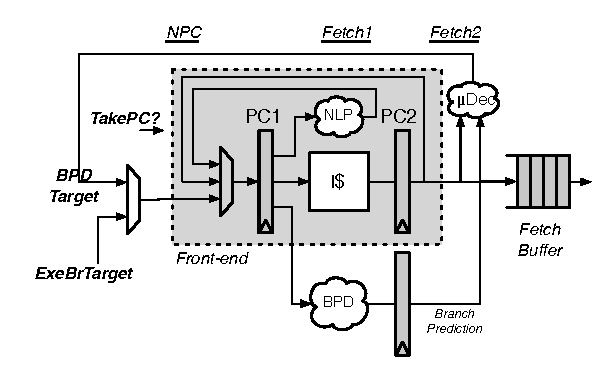
\includegraphics[scale =1] {figures/frontend}}
	\caption{ \small The Fetch Unit. The grey box is the front-end instantiated from the Rocket code base.}
	\label{fig:fetch}
\end{figure}

BOOM instantiates the Rocket core's {\em Front-end} (highlighted in grey in Fig \ref{fig:fetch}), which fetches instructions and predicts every cycle where to fetch the next instructions using a ``next-line predictor" (NLP). If a misprediction is detected in BOOM's backend, or BOOM's own predictor wants to redirect the pipeline in a different direction, a request is sent to the Front-End and it begins fetching along a new instruction path.  See Chapter \ref{chapter:bpd} for more information on how branch prediction fits into the Fetch Unit's pipeline. 

Since superscalar fetch is supported, the {\em Front-end} returns a {\em fetch packet} of instructions.  The {\em fetch packet} also contains meta-data, which includes a {\em valid mask} (which instructions in the packet are valid?) and some branch prediction information that is used later in the pipeline. 

\section{The Rocket I-Cache}

BOOM instantiates the i-cache found in the Rocket processor source code.  The i-cache is a virtually indexed, physically tagged set-associative cache. 

To save power, the i-cache reads out a fixed number of bytes (aligned) and stores the instruction bits into a register. Further instruction fetches can be managed by this register. The i-cache is only fired up again once the fetch register has been exhausted (or a branch prediction directs the PC elsewhere).  

%When a miss occurs, the cache-line is returned in smaller chunks over a parameterizable N refill cycles. The size of a refill chunk dictates the width of the instantiated memory bank. Thus, within a way, a cache-line is striped across the physical memory bank to match the incoming refill size. To minimize power, at most only one row of the memory bank is read a cycle, which dictates the maximum size of the fetch register. Thus, the i-cache (currently) does not support fetching instruction packets that straddle across a memory bank row.  Worded another way, if BOOM is parameterized to have 64 byte cache lines and the uncore returns 16 bytes per cycle over 4 cycles, 
 
The i-cache does not (currently) support fetching across cache-lines, nor does it support fetching unaligned relative to the superscalar fetch address.\footnote{This constraint is due to the fact that a cache-line is not stored in a single row of the memory bank, but rather is striped across a single bank to match the refill size coming from the uncore.  Fetching unaligned would require modification of the underlying implementation, such as banking the i-cache such that consecutive chunks of a cache-line could be accessed simultaneously.}

The i-cache does not (currently) support hit-under-miss.  If an icache miss occurs, the icache will not accept any further requests until the miss has been handled.  This is less than ideal for scenarios in which the pipeline discovers a branch mispredict and would like to redirect the icache to start fetching along the correct path. 


The front-end (currently) only handles the RV64G ISA, which uses fixed-size 4 bytes instructions. 

\section{The Fetch Buffer}

{\em Fetch packets} coming from the i-cache are placed into a {\em Fetch Buffer}.  The {\em Fetch Buffer} helps to decouple the instruction fetch front-end from the execution pipeline in the back-end. 

The instructions within a {\em fetch packet} are {\em not} collapsed or compressed - any bubbles within a {\em fetch packet} are maintained. 

The {\em Fetch Buffer} is parameterizable. The number of entries can be changed and whether the buffer is implemented as a ``flow-through" queue\footnote{A flow-through queue allows entries being enqueued to be immediately dequeued if the queue is empty and the consumer is requesting (the packet ``flows through" instantly).} or not can be toggled.  